\newpage
\section{Interfaccia Grafica}\label{sec:interfaccia-grafica}

\begin{figure}
    \centering
    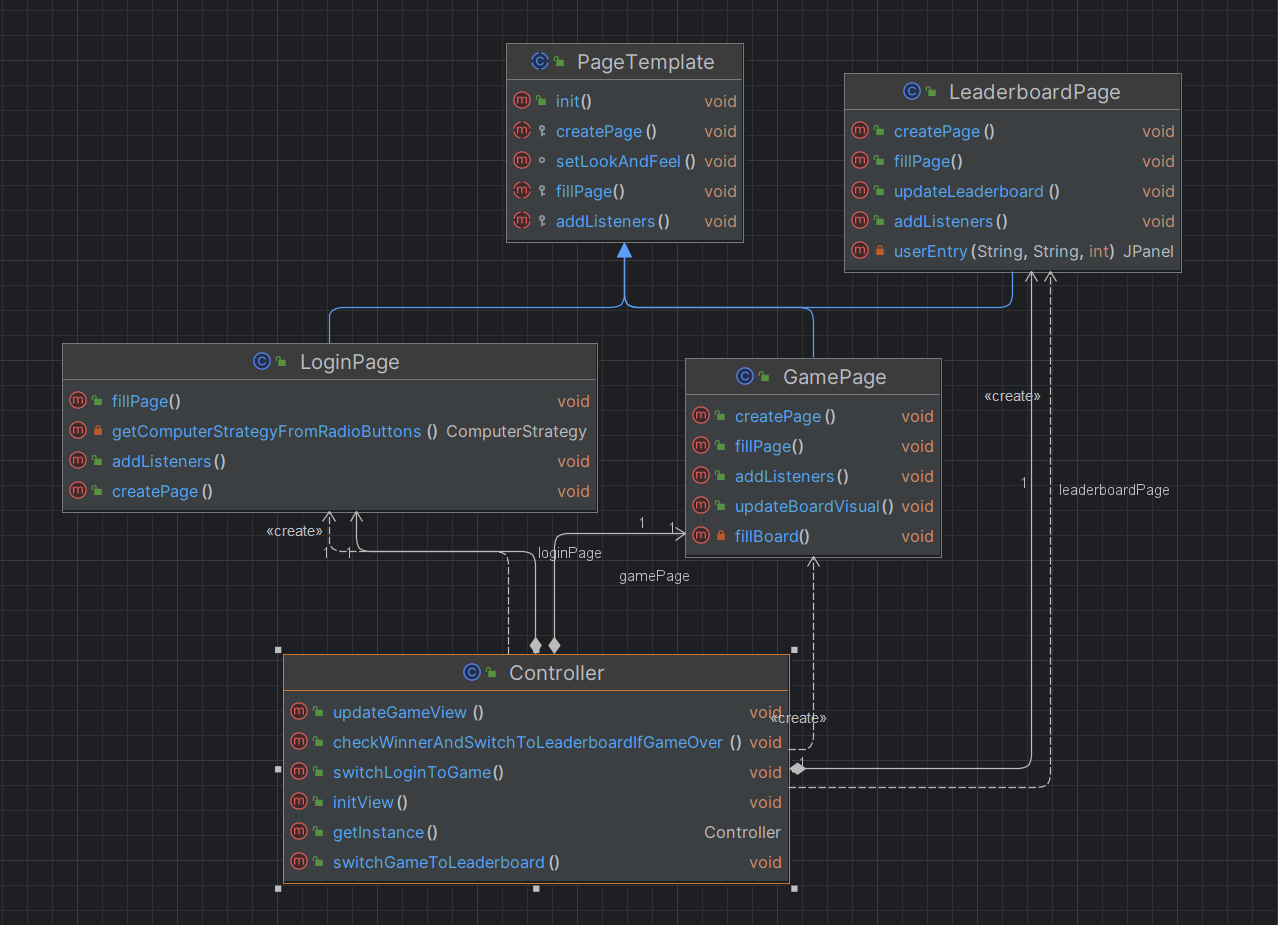
\includegraphics[scale=0.4]{img/controller-uml}
    \caption{Diagramma UML delle classi Controller e PageTemplate}
    \label{fig:controller-uml}
\end{figure}

\subsection{Template Method}\label{subsec:template-method}

L'applicazione è stata sviluppata come programma standalone con supporto grafico utilizzando la libreria di Java
\textbf{Swing}. \\
Ogni pagina dell'applicazione è creata utilizzando la classe astratta \textit{PageTemplate}, che implementa il
Design Pattern \textbf{Template Method}\cite{GoF}. \\
L'obiettivo di PageTemplate è quello di creare un unico metodo per inizializzare le pagine, in modo che la creazione
delle pagine sia analoga. \\
Il metodo di template \textit{init()} implementa la creazione delle pagine come segue:
\begin{itemize}
    \item Il metodo astratto \textit{createPage()} che include i metodi di Swing per la creazione della pagina.
    \item Il metodo \textbf{final} \textit{setLookAndFeel()} che si occupa di impostare il look and feel di ogni pagina
    allo stesso modo, non deve quindi poter essere possibile per le sottoclassi fare un @Override di questo metodo.
    \item Il metodo \textit{fillPage()}, che è un metodo di \textbf{hook}, ovvero non tutte le classi sono obbligate a
    definirlo, e ha lo scopo di riempire la pagina con elementi dinamici, generati cioè in fase di esecuzione.
    \item Il metodo \textit{addListeners()} dove le pagine possono andare a definire le operazioni da assegnare ai
    propri bottoni.
\end{itemize}

In questo caso il pattern Template Method è stato utilizzato con lo scopo di generalizzare il comportamento comune
tra le classi rappresentanti le pagine dell'applicazione, e per controllare l'estensione delle sottoclassi attraverso
il metodo di hook \textit{fillPage()}.

\begin{figure}
    \begin{verbatim}
    public abstract class PageTemplate extends JFrame {
        public final void init() {
            createPage();
            fillPage();
            setLookAndFeel();
            addListeners();
            setLocationRelativeTo(null);
            setDefaultCloseOperation(JFrame.EXIT_ON_CLOSE);
            setResizable(false);
        }

        protected abstract void createPage();

        // metodo di hook
        protected void fillPage() {
        }

        // metodo final:
        // tutte le pagine devono avere lo stesso look and feel
        final void setLookAndFeel() {
            try {
                UIManager.setLookAndFeel(
                        "com.jtattoo.plaf.hifi.HiFiLookAndFeel
                                        ");
            } catch (Exception e) {
                System.out.println(e.getMessage());
            }
        }

        protected abstract void addListeners();
    }
    \end{verbatim}
    \caption{Implementazione di Template Method attraverso la classe astratta PageTemplate}
    \label{fig:page-template}
\end{figure}

\newpage
\subsection{Controller}\label{subsec:controller}

La classe \textit{Controller} si occupa invece di gestire il flusso di operazioni relative all'interfaccia grafica. \\
Controller inizializza le diverse pagine che compongono l'applicazione richiamando i loro metodi template, dopodiché
espone dei metodi per cambiare la pagina corrente, associando al cambiamento di pagine dei comportamento opportuni. \\
In questo modo Controller non espone le istanze concrete delle singole pagine, e pertanto permette di disaccoppiare
la gestione della GUI e le transizioni tra le pagine dalla logica dell'applicazione. \\
Controller è implementato come \textbf{Singleton}\cite{GoF}, in quanto non avrebbe senso avere più gruppi di pagine attive, e
deve essere facilmente accessibile dalle altre classi, per esempio dal GameHandler quando diventa necessario aggiornare
la vista della griglia attraverso il metodo \textit{updateGameView}. \\


\subsection{Login Page}\label{subsec:login-page}

\begin{figure}
    \centering
    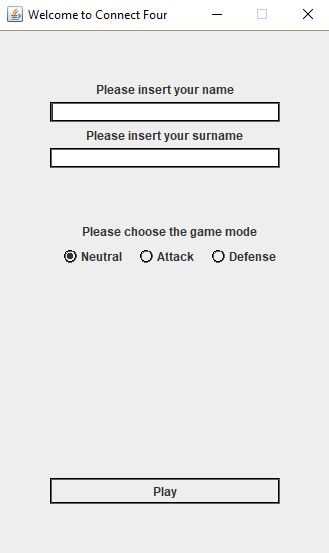
\includegraphics[scale=0.5]{img/login-page}
    \caption{Pagina di Login}
    \label{fig:login-page}
\end{figure}

La pagina di Login permette al giocatore di inserire il proprio nome e cognome e di scegliere la modalità di gioco. \\
Si occupa di controllare che sia il campo nome che il campo cognome non siano vuoti, dopodiché quando l'utente preme
il tasto \textit{Play} invia questi dati al GameHandler e comunica al Controller di cambiare pagina. \\


\newpage
\subsection{Game Page}\label{subsec:game-page}

\begin{figure}
    \centering
    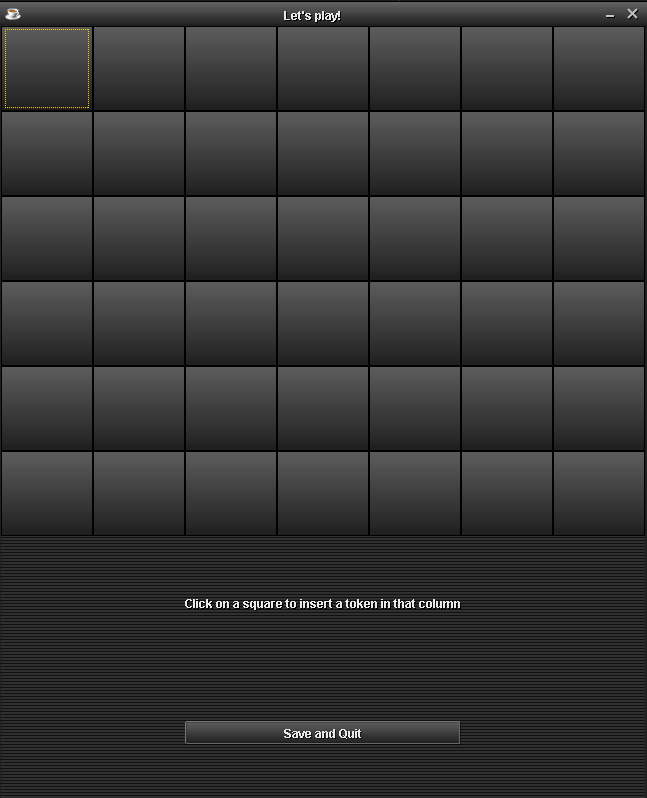
\includegraphics[scale=0.5]{img/game-page}
    \caption{Pagina di gioco}
    \label{fig:game-page}
\end{figure}

\begin{figure}
    \centering
    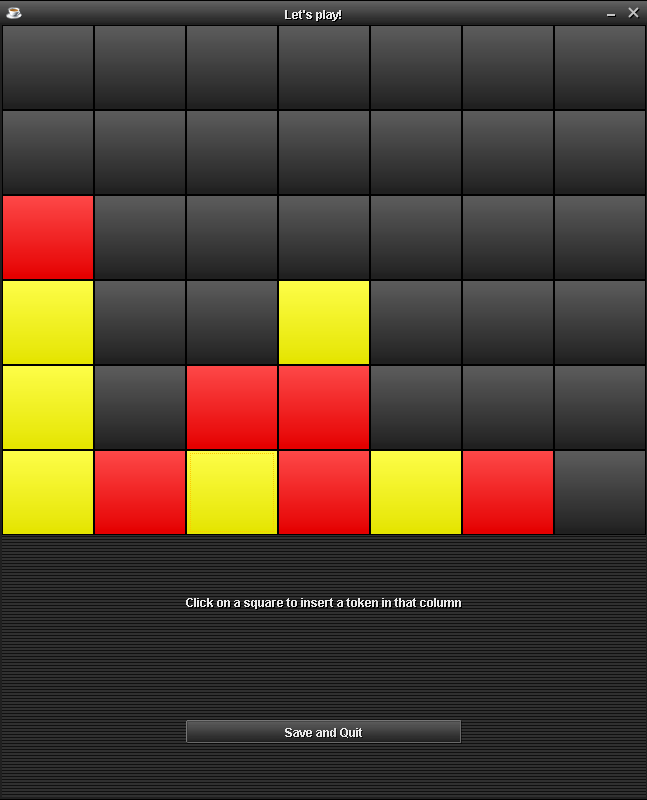
\includegraphics[scale=0.5]{img/game-page2}
    \caption{Pagina di gioco dopo aver inserito delle pedine}
    \label{fig:game-page2}
\end{figure}

La classe GamePage gestisce la pagina di gioco, la griglia viene visualizzata come una griglia di bottoni delle
stesse dimensioni. \\
Alla pressione di un bottone da parte dell'utente viene inserita una pedina in quella colonna, se vi sono quattro
pedine in fila, viene richiamato il metodo apposito del Controller per cambiare pagina alla Leaderboard Page \\
In questa pagina è anche possibile utilizzare il bottone \textit{Save and Quit} per salvare la partita, richiamando
il metodo opportuno del GameHandler, che delega la codifica della partita in un file di testo al GameLoader. \\

\newpage
\subsection{Leaderboard Page}\label{subsec:leaderboard-page}

\begin{figure}
    \centering
    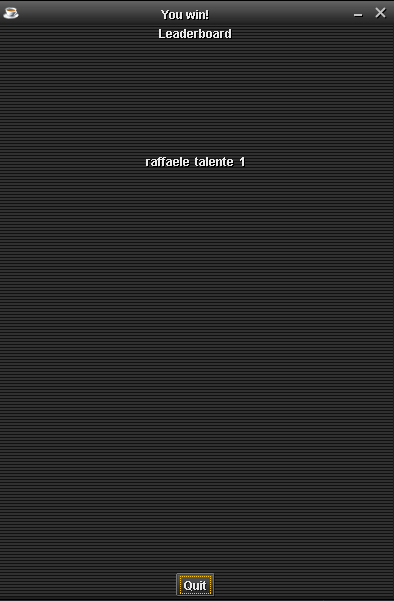
\includegraphics[scale=0.5]{img/leaderboard-page}
    \caption{Pagina di Leaderboard}
    \label{fig:leaderboard-page}
\end{figure}

\begin{figure}
    \centering
    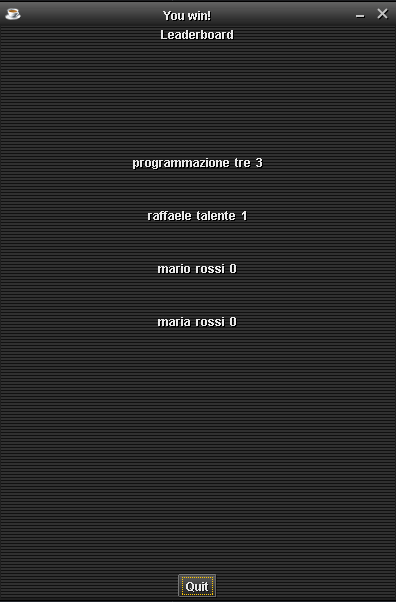
\includegraphics[scale=0.5]{img/leaderboard-page2}
    \caption{Pagina di Leaderboard con diversi utenti}
    \label{fig:leaderboard-page2}
\end{figure}

Al termine della partita, la LeaderBoard page utilizza un metodo della classe Database per ottenere i primi dieci
utenti nel database con il più alto numero di vittorie, e aggiorna opportunamente il contenuto della pagina.